%  LaTeX support: latex@mdpi.com 
%  In case you need support, please attach all files that are necessary for compiling as well as the log file, and specify the details of your LaTeX setup (which operating system and LaTeX version / tools you are using).

%=================================================================
\documentclass[journal,article,submit,moreauthors,pdftex, applsci]{Definitions/mdpi} 

% If you would like to post an early version of this manuscript as a preprint, you may use preprint as the journal and change 'submit' to 'accept'. The document class line would be, e.g., \documentclass[preprints,article,accept,moreauthors,pdftex]{mdpi}. This is especially recommended for submission to arXiv, where line numbers should be removed before posting. For preprints.org, the editorial staff will make this change immediately prior to posting.

%----------
% submit
%----------
% The class option "submit" will be changed to "accept" by the Editorial Office when the paper is accepted. This will only make changes to the frontpage (e.g., the logo of the journal will get visible), the headings, and the copyright information. Also, line numbering will be removed. Journal info and pagination for accepted papers will also be assigned by the Editorial Office.

%------------------
% moreauthors
%------------------
% If there is only one author the class option oneauthor should be used. Otherwise use the class option moreauthors.

%=================================================================
\firstpage{1} 
\makeatletter 
\setcounter{page}{\@firstpage} 
\makeatother
\pubvolume{xx}
\issuenum{1}
\articlenumber{5}
\pubyear{2019}
\copyrightyear{2019}
%\externaleditor{Academic Editor: name}
\history{Received: date; Accepted: date; Published: date}
%\updates{yes} % If there is an update available, un-comment this line

%% MDPI internal command: uncomment if new journal that already uses continuous page numbers 
%\continuouspages{yes}

%------------------------------------------------------------------
% The following line should be uncommented if the LaTeX file is uploaded to arXiv.org
%\pdfoutput=1

%=================================================================
% Add packages and commands here. The following packages are loaded in our class file: fontenc, calc, indentfirst, fancyhdr, graphicx, lastpage, ifthen, lineno, float, amsmath, setspace, enumitem, mathpazo, booktabs, titlesec, etoolbox, amsthm, hyphenat, natbib, hyperref, footmisc, geometry, caption, url, mdframed, tabto, soul, multirow, microtype, tikz

\usepackage[single=true, macros=true, xspace=true]{acro}  % For acronyms
\usepackage{cleveref} % For references
\usepackage[squaren,Gray]{SIunits}
\usepackage{subcaption}
% \usepackage{tikz}


%=================================================================
%% Please use the following mathematics environments: Theorem, Lemma, Corollary, Proposition, Characterization, Property, Problem, Example, ExamplesandDefinitions, Hypothesis, Remark, Definition, Notation, Assumption
%% For proofs, please use the proof environment (the amsthm package is loaded by the MDPI class).

%=====================================
% INPUTS
%=====================================
%% Acronym definition example using glossaries package
%% \usepackage{acro} is required
%% 
%% For a powerful usage of the acro package look at http://tex.stackexchange.com/questions/135975/how-to-define-an-acronym-by-using-other-acronym-and-print-the-abbreviations-toge

 \DeclareAcronym{auc}{
  short = AUC,
  long =  area under the curve
}

 \DeclareAcronym{bcc}{
  short = BCC,
  long =  basal cell carcinoma
}

 \DeclareAcronym{cart}{
  short = CART,
  long =  classification and regression trees
}

\DeclareAcronym{cnn}{
  short = CNN,
  long = convolutional neural network
}

\DeclareAcronym{dej}{
  short = DEJ,
  long =  dermal-epidermal junction
}

\DeclareAcronym{ert}{
  short = ERT,
  long =  extremely randomized trees
}

\DeclareAcronym{ggd}{
  short = GGD,
  long = generalized Gaussian distribution
}

\DeclareAcronym{glh}{
  short = GLH,
  long = gray level histogram
}

\DeclareAcronym{glcm}{
  short = GLCM,
  long = gray level co-occurrence matrix
}

\DeclareAcronym{lm}{
  short = LM/LMM,
  long = lentigo maligna/lentigo maligna melanoma
}

\DeclareAcronym{mil}{
  short = MIL,
  long = multiple instance learning
}

\DeclareAcronym{rcm}{
  short = RCM,
  long = reflectance confocal microscopy
}

\DeclareAcronym{roc}{
  short = ROC,
  long = receiver operating characteristic
}

\DeclareAcronym{sil}{
  short = SIL,
  long = Single-Instance Learning
}

\DeclareAcronym{svm}{
  short = SVM,
  long = Support Vector Machine
} 

%=================================================================
% Full title of the paper (Capitalized)
\Title{Computer-Aided Diagnosis classification of Lentigo Malignant through Reflectance Confocal Microscopy images}

% Author Orchid ID: enter ID or remove command
\newcommand{\orcidauthorA}{0000-0002-6449-9723} % Cendre Add \orcidA{} behind the author's name
\newcommand{\orcidauthorB}{0000-0001-9054-3719} % Mansouri
\newcommand{\orcidauthorC}{0000-0003-4479-9961} % Perrot 
\newcommand{\orcidauthorD}{0000-0002-4009-0659} % Cinotti 
\newcommand{\orcidauthorE}{0000-0003-0963-1565} % Marzani 


% Authors, for the paper (add full first names)
\Author{Romain Cendre~$^{1,*}$\orcidA{}, Alamin Mansouri~$^{1}$\orcidB{}, Jean-Luc Perrot~$^{2}$\orcidC{}, Elisa Cinotti~$^{3}$\orcidD{} and Franck Marzani~$^{1}$\orcidE{}}

% Authors, for metadata in PDF
\AuthorNames{Romain Cendre, Alamin Mansouri, Jean-Luc Perrot, Elisa Cinotti and Franck Marzani}

\address{%
$^{1}$ \quad Laboratoire ImViA (EA 7535), Université Bourgogne Franche-Comté, Dijon, France; imvia.direction@u-bourgogne.fr\\
$^{2}$ \quad Service de Dermatologie-Oncologie-Allergologie, CHU de Saint-Etienne, Saint-Etienne, France\\
$^{3}$ \quad U.O. Dermatologia, Dipartimento di Scienze Mediche, Chirurgiche e Neuroscienze, A.O.U.S. Le Scotte - Università degli Studi di Siena, Siena, Italia}

% Contact information of the corresponding author
\corres{Correspondence: romain.cendre@gmail.com}

% Abstract
\abstract{Reflectance Confocal Microscopy is an appropriate tool for diagnosis of the diagnosis of Lentigo Maligna. In comparison with Dermoscopy, this device can provide rich information as a mosaic and/or stack of images. In this particular context, the number of images by patients varies between 2 and 833 images and the finality is to separate them between Benign and Malignant classes. First, this paper evaluates classification at image-level with help of handcrafted methods issue from literature and Transfer Learning methods. Second, this work proposes patient-level supervised methods based on images decisions and compare them to multi-instance learning methods. At image-level classification, this study achieves an F1-Score of 0.83 on malignant pathologies by use of “Inception-ResNet” architecture and Linear SVM. On patient-level side, this study reach weighted F1-Score of 0.83 (Sensitivity 0.88 / Specificity 0.75) with an \ac{auc} score of 0.87 using the supervised method based dynamic threshold and achieve weighted F1-Score of 0.80 (Sensitivity 0.78 / Specificity 0.84) with an \ac{auc} score of 0.88 using the multi-instance learning method based on MI-SVM.}\par

% Keywords
\keyword{Computer-assisted diagnosis; Classification; Transfer Learning; Reflectance Confocal Microscopy; Dermatology; Lentigo}

%%%%%%%%%%%%%%%%%%%%%%%%%%%%%%%%%%%%%%%%%%
% Only for the journal Applied Sciences:
\featuredapplication{This paper focus in an enhance of the patient care and also helps practitioners to optimize their time in dermatology services through computer-assisted diagnosis software using data from \acl{rcm} devices.}
%%%%%%%%%%%%%%%%%%%%%%%%%%%%%%%%%%%%%%%%%%

%%%%%%%%%%%%%%%%%%%%%%%%%%%%%%%%%%%%%%%%%%
\begin{document}
%%%%%%%%%%%%%%%%%%%%%%%%%%%%%%%%%%%%%%%%%%

%=====================================
% INTRODUCTION
%=====================================
\section{Introduction}
These days, skin cancers are the most prevalent form of human malignancy, with an increasing incidence rate over the years. These disease affect people in their everyday life by having a heavy social impact on those affected, not only decreasing their quality of life, but also potentially becoming lethal. In addition, they have significant economic consequences, with an estimated cost of 8 billion dollars per year in the United States~\cite{Farberg2017a}, and can cause an overhelming saturation of dermatological centers. However, most of these repercussions could be avoided with an early detection and appropriate surgeries~\cite{Farberg2017a}.\par
Currently, histological examination is the gold standard to diagnose skin cancers in the clinical context. This process is relatively long: it needs to excise the concerned area, to embed the sample in paraffin, to cut it in thin slices that should be colored and to examine it by an histopathologist. However, despite its precision, this technique remains time consuming, invasive and inconvenient for doctors and patients. Consequently, several non-invasive imaging techniques were developed to help the classification of skin cancers and nowadays some of them are of common use by dermatologists. For instance, clinical photography and dermoscopy are both examples of affordable and intuitive techniques largely exploited by dermatologist. Dermoscopy tends to replace clinical photography as it significantly improves the quality of diagnosis made by the experts, thanks to acquisition of high magnification images of the skin~\cite{Sinz2017}.\par
These days, research papers on dermatology focus on dermoscopy modality to perform an automatic classification of lesions. Most of them obtain acceptable results on melanocytic pathologies~\cite{Iyatomi2010}. Older methods focus on finding the most pertinent combination of preprocessing steps and hand-crafted features to be used in a machine learning scheme~\cite{Rastgoo2015,Pathan2018}. In contrast, most recent methods are using deep learning approaches and shows impressive results in this discipline~\cite{Esteva2017}. In that particular work, the authors use an Inception-V3 architecture pretrained on the “ImageNet” database~\cite{Deng2008} and fine-tune this model on a dataset of 129,450 clinical images containing 2,032 different skin lesions and distributed across 757 classes. They realise the classification at different taxonomy levels and achieve at the first level of classification (Non-neoplastic versus Benign versus Malignant) an accuracy of 72.1$\pm$0.9\% against 66.0\% on a subset of these data by specialists.\par
However, Dermoscopy imaging device only provide a surface and chromatic information. To overcome these, the \ac{rcm} modality is another type of imaging technique used by dermatologists providing high resolution images of the skin at micrometer scale. Furthermore, this modality can provide structural information at different depths of the skin by adjusting the wavelength properties and the focal point~\cite{Kolm2012}. Nowadays, this tool has a superior diagnostic accuracy compared to dermoscopy both for melanocytic and non melanocytic skin tumors~\cite{Haroon2017, Dinnes2018, Lupu2019}. In opposition to previous modalities, \ac{rcm} remains expensive, although the number of users continues to increase~\cite{Batta2015} and recent works have started to improve the portability of \ac{rcm} devices~\cite{Freeman2018}.\par
By contrast, relatively less work have been published on \ac{rcm} modality by use of computer vision techniques despite their promising results in a clinical context. The use of artificial intelligence could be particularly useful for RCM images because their evaluation by  dermatologists is time consuming. Indeed, differently form dermoscopy, many RCM images should be acquired for each skin lesion. Many studies on computer vision focus on understanding these images by predicting the position in the skin layer \cite{Somoza2014,Hames2016}, by using stacks of 3D data provided by this modality. Some other works are describing the structural components of the skin \cite{Gareau2010} and few of them are classifying pathologies from that specific modality. One of these paper~\cite{Wiltgen2008} is quite similar to the problem explored in this work, and suggests several images descriptors to serve a classification task. These authors introduce two methods using frequency representation: the first one based on Fourier transform and second one based on wavelet representation by use of Daubechies 4. The intuition behind spectral representation is to extract information at different frequency level giving information about smoothness or complex structures inside the images, and to be robust to rotations and translations as pathologies are non oriented. The second category of descriptors they used is based on spatial features by use of \ac{glh} and \ac{glcm} statistical descriptors. The statistical descriptors computed from \ac{glcm} are issue from a previous work~\cite{Haralick1973}. Finally, the authors proceed to classification of images by using different image parts at multiple sizes and proceed to CART classification. In a two class situation, this paper reaches an accuracy of 96\% for Nevi detection and 97\% for Melanoma pathologies by applying a wavelet extraction and \ac{cart} classification on a sub part of image of 256*256 pixels. Another paper is more relevant as the authors follow the same purpose as this work by suggesting a way to classify solar lentigo pathologies by use of the previous wavelet decomposition, and by fitting the decomposition values to a \ac{ggd} to reduce the amount of variables~\cite{Halimi2017a}. They also suggest that only one variable and only one scale decomposition are relevant for solar lentigo detection. This method was applied to 45 subjects with healthy skin or solar lentigo and achieved a sensitivity of 81.4\% and specificity of 83.3\%.\par
The scope of this work is to detect the malignant tumors and particularly \ac{lm} (the most common type of facial melanoma) in \ac{rcm} images and to reach from these images a diagnosis on patient-level to help specialists. The previous feature extraction methods and extraction through different \ac{cnn} architecture are first investigated. As wavelet decomposition and reduction through \ac{ggd}~\cite{Halimi2017a} were shown irrelevant in our data context~\cite{Cendre2019a}, this work do not focus on any of these methods. Then comparison over several classification models on full size images is conducted to estimate the relevance of these methods.\par
Next parts of this paper are organized as follows. The \Cref{sec:material} covers the data by giving details about their composition, the features extraction methods implemented and the process used to compute image-level and patient-level decision. Then \Cref{sec:results} displays all the results and provide an analysis on them, and finally reach the \Cref{sec:conclusions} for conclusion of this work and draw some perspectives.\par
 
%=====================================
% Materials
%=====================================
\section{Materials and Methods}
\label{sec:material}

%=====================================
% DATA
%=====================================
\subsection{Data}
\label{sec:data}
The data from this paper are originally issue from a previous clinical study~\cite{Cinotti2018} that performs comparison between dermoscopy and \ac{rcm} modalities in the diagnosis of benign lesions such as solar lentigo and malignant tumors by focusing essentially on \ac{lm}. Theses images were acquired by three specialists, experts of non invasive skin imaging tools, by use of the hand-held VivaScope 3000® camera which uses a laser with a wavelength at \unit{830}{\nano\meter} and images up to \unit{250}{\micro\meter} of depth. In addition, this data include lesions that can highly mislead dermatology specialists.\par
Only images considered relevant for the diagnosis by two out of the three investigators were kept, at different depths of the skin : epidermis, \ac{dej} and dermis. However, most of the information was acquired at the \ac{dej}. Each \ac{rcm} image corresponds to a horizontal \unit{920}{\micro\meter} x \unit{920}{\micro\meter} section of the skin at a selected depth with a lateral resolution of \unit{1}{\micro\meter} and axial resolution of \unit{3-5}{\micro\meter}. For specifications, these images have a spatial resolution of 1000*1000 pixels with a quantification on single 8 bits channel.\par
Also, the relative position between images of a single patient is unknown, and could not bring any further knowledge in the next part of this work. Furthermore, available metadata about patient age is not used as the purpose of this work is to evaluate relevance of image classification techniques, but was initially given to experts during their assessments.\par
This data include 223 patients, for a total of 7846 \ac{rcm} images varying between 2 and 833 images per patient (with mean of 35 and standard deviation of 64). For each patient, the data provide an histopathology diagnosis that serve as ground truth and is distributed as follows:
\begin{itemize}  
\item 135 patients had “Malignant” tumors: 115 \ac{lm} and 20 \ac{bcc}.
\item 88 patients had “Benign” tumors: mainly represented by solar lentigines.
\end{itemize}
Also, the study~\cite{Cinotti2018} evaluates 21 experts and they achieve a mean sensitivity of 80\% and specificity of 81\% with an \ac{auc} score of 0.89 for the detection of \ac{lm}.\par
In order to reduce the imbalancement of the data, 28 additional benign tumors are also provided by dermatologist, that varies between 4 and 103 images per tumor (608 images in total). These new patients are only considered for a training purpose and are not taken into account into \Cref{sec:results}.\par
In addition, this data does not provide any information on individual images. As these annotations are required in next part of the work, each of these images were annotated by a specialist, with the help of a graphical interface designed for this purpose. Whereas patient labels are “Benign” or “Malignant”, some images cannot be classified into this two categories because they do not contain any of these pathology signs. For this particular reason, a “Healthy” label was introduced to characterize them. The \Cref{fig:data} give and overview of these different data. As this study focus only on binary classification of malignant pathologies against the rest, an annotation hierarchy was defined as following:
\begin{itemize}  
\item “Malignant” label : an image with at least some malignant tissues. 
\item “Benign” label : an image with no malignant tissues (either “Benign” and “Healthy”). 
\end{itemize}
These annotate images represent 5431 images, equitably divided between men and women. The “Malignant” labels account for 46\% of annotate images while “Benign” represent 54\%.\par
\begin{figure}[h]
    \begin{center}
        \includegraphics[width=\linewidth]{Figures/Data.pdf}
        \caption{In this figure, several examples of images related to the three different types of tissue: “Healthy”, “Benign” and “Malignant”.}
        \label{fig:data}
    \end{center} 
\end{figure}\par

%=====================================
% Features
%=====================================
\subsection{Feature extraction methods}
\label{sec:features}
In order to achieve the classification of the data, a reduction of the image information image need to be performed into new feature space able to distinguish either “Malignant” or “Benign” images types. According to the dermatologists, the texture plays an important role in the differentiation of the tissues types. First part of this section focus on handcrafted feature extractors base on texture from a previous work~\cite{Wiltgen2008}. Then, the deep extraction methods applied to this context and inspired by a previous work on Dermoscopy images~\cite{Esteva2017} are detailed. All feature extraction methods are listed in \Cref{tab:features_methods}, and next parts follow this table structure.\par
\begin{table}[h]
    \centering
    \begin{tabular}{lll}
    \hline
    \textbf{Category}                   &  \textbf{Name}                & \textbf{Features number}  \\ \hline
    \multirow{2}{*}{Spatial}            &  Haralick                     & 12                        \\ \cline{2-3} 
                                        &  \ac{glh}+\ac{glcm}           & 17                        \\ \hline 
    \multirow{2}{*}{Frequency}          &  Fourier                      & 38                        \\ \cline{2-3} 
                                        &  Wavelet                      & 39                        \\ \hline
    \multirow{5}{*}{Transfer Learning}  &  VGG-16                       & 512                       \\ \cline{2-3} 
                                        &  Inception-V3                 & 2048                      \\ \cline{2-3} 
                                        &  ResNet                       & 2048                      \\ \cline{2-3} 
                                        &  Inception-ResNet             & 1536                      \\ \hline
    Fine Tuning                         &  ResNet                       & 2048                      \\ \hline
    \end{tabular}
    \caption{The list of all features extraction methods performed in this paper and their associated extracted number of features.}
    \label{tab:features_methods}
\end{table}\par
The “Spatial” extraction methods are based on spatial patterns of pixels, by use of \ac{glh} and \ac{glcm}. The method named “Haralick” refers to previous work based on texture features~\cite{Haralick1973} and use \ac{glcm} concept by computing on them twelve statistical characteristics listed in \Cref{tab:histogram_features} - \ac{glcm} Features column. These characteristics are extracted along horizontal, vertical and two diagonals, then a mean is computed overall these axis as the tissues are non oriented in the space, and to reduce the number of features. A second method from previous work~\cite{Wiltgen2008}, called in this paper “\ac{glh}+\ac{glcm}”, expand twelve first initial characteristics of Haralick and add five others based on \ac{glh}. In total 17 features are extracted for each image, all statistical properties extracted are listed in \Cref{tab:histogram_features}. The Haralick features extraction is perform using the “Mahotas” library~\cite{coelho2012mahotas} and histogram features extraction is compute with help of “Scipy” library~\cite{Jones2001}.\par
\begin{table}[h]
    \centering
    \begin{tabular}{ll}
        \hline
        \textbf{\ac{glcm} Features}& \textbf{\ac{glh} Features}     \\ \hline
        Angular Second Moment      & Mean value                     \\
        Difference Moment          & Mean square deviation          \\
        Correlation                & Skewness                       \\
        Sum of Squares             & Kurtosis                       \\
        Inverse Difference Moment  & Entropy                        \\     
        Summed Average             &                                \\    
        Sum Variance               &                                \\    
        Entropy                    &                                \\    
        Sum Entropy                &                                \\    
        Difference Entropy         &                                \\    
        Measure of Correlation 1   &                                \\  
        Measure of Correlation 2   &                                \\ 
    \end{tabular}
    \caption{Statistical measures issue respectively from \ac{glcm} and \ac{glh}, and extracted in order to perform “Spatial” extraction methods.}
    \label{tab:histogram_features}
\end{table}\par
A second category of extraction methods, named “Frequency”, identifies a set of methods based on frequency approaches. First method of this category is called “Fourier” and is based on Fourier Transform. The main idea is to provide different levels of information as high frequency refer to high contrast parts and low frequencies to homogeneous areas in the image. As the spectrum is symmetric around the origin, only half of this spectrum is considered for the purpose of computational efficiency. Then a mean value is computed over all the coefficients located at the same radius distance from the origin, at 22 different radius sizes between 0 and the diagonal size of the image. A previous paper~\cite{Smach2008a} also show relevance of this method in textural images context. Finally, 16 constant directions are taken from origin of the power spectrum, and a mean value is computed on each of them~\cite{Wiltgen2008} (see \Cref{fig:handcrafted}~-~a)~). The second method of this category is called “Wavelet” in this work and is based on Wavelet transform by using a decomposition based on a Daubechies 4 that provide quite fine localisation properties~\cite{Wiltgen2008}. This decomposition is made at five scales, and only the four last scales are consider to compute coefficients  (see  \Cref{fig:handcrafted}~-~b)~). For each of them, three statistical measures are computed: the standard deviation, the energy and the entropy.\par
\begin{figure}[h]
    \begin{center}
        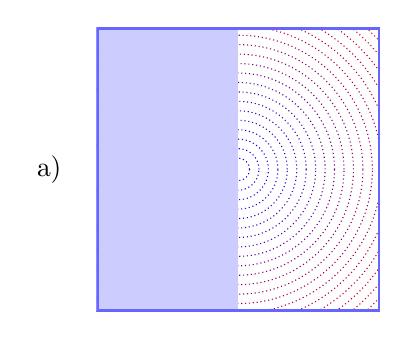
\begin{tikzpicture}[scale=1.2]
            \node[] at (-2, 0) {a)};
            \begin{scope}
                \clip (-1.5, -1.5) rectangle (1.5, 1.5);
                \foreach \cRadius in {1, ..., 22}
                    \pgfmathsetmacro\cColor{\cRadius/22*100} %22-22}
                    \draw[red!\cColor!blue, densely dotted] (0, 0) circle (0.02+\cRadius*0.1); 
                    
                \fill[blue!20] (-1.5, -1.5) rectangle (0, 1.5);
                \draw[blue!60, ultra thick] (-1.5, -1.5) rectangle (1.5, 1.5);
            \end{scope}
        \end{tikzpicture}
        \qquad
        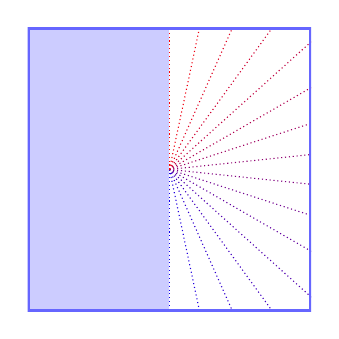
\begin{tikzpicture}[scale=1.2]
            \begin{scope}
                \clip (-1.5, -1.5) rectangle (1.5, 1.5);
                \foreach \cAngle in {1, ..., 16}
                    \pgfmathsetmacro\cColor{\cAngle/16*100}
                    \draw[red!\cColor!blue, densely dotted] (0, 0) -- (\cAngle* 180 / 15 -102:3); 
                \fill[blue!20] (-1.5, -1.5) rectangle (0, 1.5);
                \draw[blue!60, ultra thick] (-1.5, -1.5) rectangle (1.5, 1.5);
            \end{scope}
        \end{tikzpicture}
        \qquad
        \vrule
        \qquad
        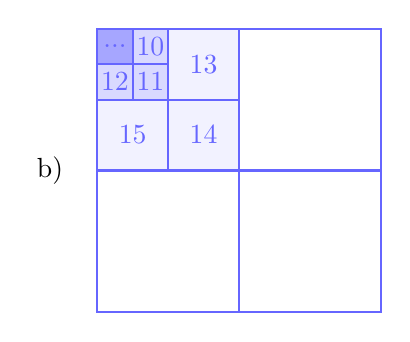
\begin{tikzpicture}[scale=1.2]
            \node[] at (-2, 0) {b)};
            % First level
            \draw[blue!60, thick] (-1.5, -1.5) rectangle (0, 0);
            \draw[blue!60, thick] (0, -1.5) rectangle (1.5, 0);
            \draw[blue!60, thick] (0, 0) rectangle (1.5, 1.5);
            % Second level
            \filldraw[blue!60, fill=blue!5, thick] (-1.5, 0) rectangle (-0.75, 0.75) node[pos=.5] {15};
            \filldraw[blue!60, fill=blue!5, thick] (-0.75, 0) rectangle (0, 0.75) node[pos=.5] {14};
            \filldraw[blue!60, fill=blue!5, thick] (-0.75, 0.75) rectangle (0, 1.5) node[pos=.5] {13};
            % Third level
            \filldraw[blue!60, fill=blue!15, thick] (-1.5, 0.75) rectangle (-1.5+0.375, 0.75+0.375) node[pos=.5] {12};
            \filldraw[blue!60, fill=blue!15, thick] (-1.5+0.375, 0.75) rectangle (-1.5+0.75, 0.75+0.375) node[pos=.5] {11};
            \filldraw[blue!60, fill=blue!15, thick] (-1.5+0.375, 0.75+0.375) rectangle (-1.5+0.75, 0.75+0.75) node[pos=.5] {10};
            \filldraw[blue!60, fill=blue!35, thick] (-1.5, 0.75+0.375) rectangle (-1.5+0.375, 0.75+0.75) node[pos=.5] {...};
        \end{tikzpicture}
    \end{center}
    \caption{On the left, the feature extraction process from Fourier transform, first by drawing circles mask (22 in total) then taking directions (16 in total). On the right, the wavelet decomposition described with applied measure on 0-16.}
    \label{fig:handcrafted}
\end{figure}\par
The third category of methods investigated on deep learning methods and more specifically on \ac{cnn}, which are known to be well-suited methods for image classification, thanks to robust feature patterns~\cite{Pathan2018}. Many architectures were used to deal with ImageNet challenges and their associated performance analyzed~\cite{Canziani2016}. Instead of training this network from scratch, as we have data constraints and also computational constraints, we choose a Domain Adaptation approach of these models. Most of papers are dealing with \ac{cnn} trained on ImageNet~\cite{Deng2008} as this database contains thousand of classes and more than 14 millions of images, meaning that extracted features from these networks can be used in various fields. As discussed by~\cite{Litjens2017}, Inception-V3 architecture pre-trained on ImageNet is supposed to be the most relevant for medical application. As \ac{rcm} images can be of various form and can contain specifics details compared to other image modalities, this research compares most famous \ac{cnn} architectures: VGG-16~\cite{Simonyan2014}, Inception-V3~\cite{Szegedy2015}, ResNet~\cite{He2016} and Inception-ResNet~\cite{Szegedy2017}, performing respectively 71\%, 76\%, 78\% and 80\% of accuracy on ImageNet database~\cite{Canziani2016}. This method involves usage of Transfer Learning, by removing the last layers devoted to the classification task, in order to get a new representation of images data as features. Furthermore, in order to reduce the number of features provided by previous step, a global pooling layer based on maximum of each activation layer is performed. For convenience, this whole method will be called “Transfer Learning” in the next paragraphs and name of respective networks are used. The \ac{cnn} computation was implemented using the “Keras” library~\cite{chollet2015keras}.\par

%=====================================
% IMAGE LEVEL
%=====================================
\subsection{Image-level decision}
\label{sec:image_decision}
The image-level decision is the first level of classification achieved in this study, in which image classification must be carried out under the two classes “Malignant” as positive class and “Benign”. In order to satisfy this objective, the process consists in using the image as a single instance having several discriminant characteristics and sufficient information to allow their classification. As formulated by \cite{foulds_frank_2010}, such a problem can be set as a pair \(\{X|y\}\), 
in which \(X=\{x_1,x_2,\ldots,x_n\}\) is a vector characteristics in which \(n\) is the number of features and \(y\) the associated label. The task consists in finding the existing relationship between \(X\) and \(y\), using a classification process.\par 
To achieve this task, an extraction method (see \Cref{sec:features}) is applied on images depending on the currently evaluated method, then the features are normalized based on a standard score computation to make the classification task more accurate and robust~\cite{Graf2001}. This scaling is computed by subtracting the mean, and then dividing by the standard deviation. The \Cref{fig:image_process} scheme provides an overview of this process.\par
\begin{figure}[h]
    \begin{center}
        \includegraphics[width=0.8\linewidth]{Figures/Process_Image.pdf}
        \caption{Classification process performed on \ac{rcm} images. The “Extraction” box refers to one of the Feature Extraction methods mentioned in \Cref{sec:features}. 
        The “Fit Model” and “Prediction” boxes are related respectively to training and inference steps of one of the model discussed in \Cref{sec:image_decision} respectively trained and infered. Testing set is predicted along two classes: “Benign” and “Malignant”.}
        \label{fig:image_process}
    \end{center} 
\end{figure}\par
Finally, the classification is performed on scaled features using different models. In a first time, \ac{cart} are investigated as they are previously study in the same data context~\cite{Wiltgen2008}. In a second time, as our number of features can be huge due to Transfer Learning methods, \ac{ert} models are also used as an extension of \ac{cart}~\cite{Geurts2006}. Lastly, \ac{svm} models are evaluated known to be suitable in multiples contexts~\cite{Smach2008a,Kose2016b}. As the relation between the features and expected outputs can be complex, \ac{svm} models are compared over linear and RBF kernels.\par
In addition, to provide best performance on each of these models, a search on their optimum hyperparameters is realized (see \cref{tab:image_hyperparameters}).\par
\begin{table}[]
    \centering
    \begin{tabular}{lll}
    \textbf{Name}                   & \textbf{Parameter}& \textbf{Values}               \\ \hline
    \multirow{2}{*}{\ac{cart}}      & Maximum depth     & [3, $\infty$]                 \\ \cline{2-3}
                                    & Criterion         & [Gini, Entropy]               \\ \hline 
    \multirow{2}{*}{\ac{ert}}       & Maximum depth     & [3, $\infty$]                 \\ \cline{2-3}
                                    & Criterion         & [Gini, Entropy]               \\ \hline 
    \ac{svm} Linear                 & C                 & [0.01, 0.1, 1, 10, 100, 1000] \\ \hline
    \multirow{2}{*}{\ac{svm} RBF}   & C                 & [0.01, 0.1, 1, 10, 100, 1000] \\ \cline{2-3}
                                    & Gamma             & [0.01, 0.1, 1, 10, 100, 1000] \\ \hline 
    \end{tabular}    
    \caption{List of all classification models performed in this study and their referring evaluated hyper-parameters.}
    \label{tab:image_hyperparameters}
\end{table}\par


%=====================================
% PATIENT LEVEL
%=====================================
\subsection{Patient-level decision}
\label{sec:patient_decision}
This part is dedicated on different ways to achieve the classification at patient-level under the same two categories as previously: “Malignant” as positive class and “Benign”. With this assumption, a patient should be considered as “Malignant” if at least one images is considered as “Malignant”. Additionally, this part needs to consider the varying number of samples by patient (as reminder, the number of instances per patient can varies between 2 and 833 images).\par
In order to achieve this, the best combination between the feature extraction method and the classification model from \Cref{sec:image_decision} is used. The classification model provides two types of information over each image: the score issues from prediction probabilities and the decision (i.e.\ the class that achieve the best probability). In both cases, due to varying number of images by patients, the information needs to be transform into constant size matrices to take a decision on existing and over new patient. At score level, the structure is composed of patients, images and scores of classes and transform into a new matrix of size P*C where P is number of patients and C the number of classes. Then a dynamic threshold is adjust on the positive class that maximizes the chosen metric. Multiple strategies are used to achieve this:
\begin{itemize}
\item Mean - allows to keep the contribution of each instance on the patient
\item Maximum - keep the best confidence prediction as the trusted one.
\end{itemize}
At decision level, the structure is composed by structure combining patients, images and scores of classes and transform into a new matrix of size P*C where P is number of patients and C the number of classes. Also, C refers to the probability vector of each decision between 0 and 1. 
\begin{itemize}
\item At Least One - at least one positive decision to consider as positive (initial assumption)
\item Dynamic - find a dynamic threshold that minimize false positive decisions.
\end{itemize}
For a global overview of the processing scheme of this method, refers to \Cref{fig:decision_process}.
\begin{figure}[h]
    \begin{center}
        \includegraphics[width=\linewidth]{Figures/Process_Decision.pdf}
        \caption{Classification process performed on \ac{rcm} patients, in which first part of the process remains the same as \cref{sec:image_decision}. The “Fit Model” and “Prediction” boxes refers to the decision and score level methods discussed in \Cref{sec:patient_decision}. Testing set is predicted along the patients over “Benign” and “Malignant” classes.}
        \label{fig:decision_process}
    \end{center} 
\end{figure}\par
In a second time, some \ac{mil} concept are implemented in this part as they are fitting the problematic: a patients is constitutive of several instances (consider it as a bag) and a positive instance suppose that the patient should be positive. Furthermore, only the patient label is known and the annotation step of individual images is time consuming. Such a problem can be set as a pair \(\{X|y\}\), in which \(X=\{X^1,X^2,\ldots,X^b\}\) be a bag containing \(b\) instances and each \(X^b\) formulated as following \(X^b=\{x^b_1,x^b_2,\ldots,x^b_n\}\) in which \(n\) is the number of features and \(y\) the patient label~\cite{foulds_frank_2010}. Regarding of this context, two ideas are developed in next paragraphs. In a first time, a \ac{sil} are used in which a bag is considered as negative if all instances are considered negative and positive if at least one of the instances has a positive label, that fit our initial formulation of patient label. In a second time, the MI-SVM are an extension of \ac{svm} upon \ac{mil} theory and are employed in these due to results of \Cref{sec:image_decision}. These experiments are configured to perform with a linear kernel due to observation made over experiments of \Cref{sec:image_decision}. This part experiments are implemented using the “MISVM” library~\cite{Doran2014}.\par
In addition, to provide best performance on each of these models, a search on their optimum hyperparameters is realized (see \cref{tab:patient_hyperparameters}). In addition, for simplicity of next sections, this paper refers to \cref{tab:patient_hyperparameters} - Name column to name each method.\par
\begin{table}[]
    \centering
    \begin{tabular}{llll}
    \textbf{Category}               & \textbf{Name}     & \textbf{Parameter}& \textbf{Values}                                   \\ \hline
    \multirow{2}{*}{Score}          & Mean              & \multirow{2}{*}{-}& \multirow{2}{*}{[]}                               \\ \cline{2-2}
                                    & Maximum           &                   &                                                   \\ \hline 
    \multirow{2}{*}{Decision}       & At Least One      & \multirow{2}{*}{-}& \multirow{2}{*}{[]}                               \\ \cline{2-2}
                                    & Dynamic           &                   &                                                   \\ \hline 
    \multirow{2}{*}{\ac{mil}}       & \ac{sil}          & \multirow{2}{*}{C}& \multirow{2}{*}{[0.01, 0.1, 1, 10, 100, 1000]}    \\ \cline{2-2}
                                    & MI-SVM            &                   &                                                   \\ \hline 
    \end{tabular}    
    \caption{List of all classification models and referring evaluated hyper-parameters.}
    \label{tab:patient_hyperparameters}
\end{table}
\par


%=====================================
% RESULTS
%=====================================
\section{Results}
\label{sec:results}

\subsection{Validation and evaluation metric}
The validation protocol remains the same for each of these experiments, based on a nested cross-validation known to be less bias than a simple cross validation~ scheme\cite{Cawley2010}. This process allows to 1) cross validate hyper-parameters and 2) evaluate the prediction models objectively. Each of the cross-validation steps is based on K-Fold strategy with $k$ value of 4 on testing loop and 2 on validation loop. Also, each folds are patients separated and balanced as best as possible based on images labels. In order to evaluate objectively, each data cluster remains the same for experiments in a same section (refers to \cref{sec:image_decision} and \cref{sec:patient_decision}). Moreover, each experiments are validated and evaluated using an F1-Score metric, as it is statistically suitable for unbalanced populations compared to accuracy metric, and represent in a single value recall and precision information. In addition, a standard deviation is compute to achieve an analysis of the stability of models along the nested cross-validation. For this purpose we use the “Scikit Learn” library for Machine Learning classification, validation and metric~\cite{pedregosa2011scikit}.\par

\subsection{Experiments and Discussion}
The results of \Cref{sec:image_decision} on image-level decisions are performed only on the labeled images and are listed in \cref{tab:image_results}. The most suitable handcrafted extraction methods is based on the “Wavelet” method combined with the Linear \ac{svm} model and reach a F1-Score score of 0.74 with quite stable performance of 0.04. In general, all the handcrafted methods perform in quite similar and stable way, varying between 0.69 and 0.74 for F1-Score and 0.03 and 0.06 for deviation. In addition, Transfer Learning based features extraction reach higher scores on the Linear \ac{svm} model, in particular with “Inception-ResNet” architecture achieving a weighted F1-Score of 0.83 with a deviation of 0.04. On this similar model, Transfer Learning features extraction methods varies between 0.77 and 0.83 with deviation range between 0.02 and 0.04. In opposition, all these architectures performed poorly on RBF \ac{svm} model, but can be explained by an excessive number of features that result in an overfitting despite of the cross validation of hyper-parameter “C”. The “VGG-16” architecture is performing better with only 512 features than the remaining architecture providing 1536 or 2048 features. About classification model based on Trees, no such difference is attest between \ac{cart} and \ac{ert} on handcrafted methods, but a notable difference is found when using Transfer Learning extraction method. This can due to the huge number of features as related to RBF \ac{svm} model. As a partial conclusion, the rest of this article keeps only the best combination with “Inception-ResNet” as feature extraction methods and Linear \ac{svm} classification model.\par
\begin{table}[h]
    \centering
    \begin{tabular}{llcccc}
    \multicolumn{2}{c}{}                                                &\multicolumn{4}{c}{\textbf{Classifier type}}                                                           \\ \cline{3-6}
    \multicolumn{2}{c}{}                                                &\textbf{\ac{cart}}     &\textbf{\ac{ert}}          &\textbf{Linear \ac{svm}}   &\textbf{RBF \ac{svm}}  \\ \hline
    \multirow{8}{*}{\textbf{Features}}  &\textbf{Haralick}              &0.71$\pm$0.04          &0.71$\pm$0.05              &0.71$\pm$0.05              &0.70$\pm$0.06          \\ \cline{2-6} 
                                        &\textbf{\ac{glh}+\ac{glcm}}    &\textbf{0.71$\pm$0.03} &0.71$\pm$0.05              &0.70$\pm$0.05              &0.71$\pm$0.04          \\ \cline{2-6} 
                                        &\textbf{Fourier}               &0.69$\pm$0.05          &0.70$\pm$0.04              &0.72$\pm$0.03              &0.69$\pm$0.06          \\ \cline{2-6} 
                                        &\textbf{Wavelet}               &0.69$\pm$0.03          &0.73$\pm$0.04              &0.74$\pm$0.04              &\textbf{0.72$\pm$0.03} \\ \cline{2-6} 
                                        &\textbf{VGG-16}                &0.63$\pm$0.03          &0.77$\pm$0.05              &0.77$\pm$0.03              &0.65$\pm$0.20          \\ \cline{2-6} 
                                        &\textbf{Inception-V3}          &0.64$\pm$0.04          &0.79$\pm$0.04              &0.80$\pm$0.03              &0.44$\pm$0.04          \\ \cline{2-6} 
                                        &\textbf{ResNet}                &0.63$\pm$0.04          &0.79$\pm$0.04              &0.79$\pm$0.02              &0.44$\pm$0.04          \\ \cline{2-6} 
                                        &\textbf{Inception-ResNet}      &0.64$\pm$0.04          &\textbf{0.80$\pm$0.04}     &\textbf{0.83$\pm$0.04}     &0.45$\pm$0.03          \\ \hline 
    \end{tabular}    
    \caption{List of results based on combinations of features extraction methods from \Cref{sec:features} and classification models from \Cref{sec:image_decision} evaluated over a weighted F1-Score of Benign and Malignant classification.}
    \label{tab:image_results}
\end{table}
This paragraph focus on methods implemented to reach the patient diagnosis (see \Cref{sec:patient_decision}) and performs on the initial \ac{rcm} data (including unlabelled images) on which specialists were previously evaluated~\cite{Cinotti2018}. All these experiments results are listed in \Cref{tab:patient_results} and discussed in next sentences. In the first place, the methods based on decision varies between 0.61 and 0.84 for F1-Score from Malignancy. The “At Least One” method achieve poor performance due to insufficient result on “Benign” class. This actual problem is solved by use of the “Dynamic” method based on dynamic activation threshold over decisions to minimize the risks of false positive, but result in an ethic consideration of this method on clinical context. In the second place, the methods based on score are quite equivalent and varies between 0.76 and 0.83 for F1-Score on Malignancy. In opposition with these results, standard deviations remain reasonable varying between 0.03 and 0.06. Finally, \ac{mil} are also evaluated, and shown important difference between \ac{sil} and MI-SVM. Indeed, the \ac{sil} assumption have similar results with the Decision based “At Least One” method, due to an insufficient discrimination capacity on the same “Benign” class. Contrariwise, the MI-SVM obtain some good results performing with F1-Score of 0.82. Both methods are quite stable with a deviation that varies only between 0.02 and 0.04. Poor results on the “At Least One” and \ac{sil} methods can be due to lack of discriminate information provided by “Inception-ResNet” for these methods.\par
\begin{table}[h]
    \centering
    \begin{tabular}{lllll}
                                &                   & \multicolumn{3}{c}{\textbf{Malignancy - F1-Score}}                    \\ \hline
    \textbf{Category}           & \textbf{Name}     & \textbf{Weighted}     & \textbf{Benign}       & \textbf{Malignant}    \\ \hline
    \multirow{2}{*}{Decision}   & At Least One      & 0.61$\pm$0.06         & 0.32$\pm$0.07         & 0.79$\pm$0.05         \\ \cline{2-5} 
                                & \textbf{Dynamic}  & \textbf{0.84$\pm$0.03}& \textbf{0.78$\pm$0.07}& \textbf{0.87$\pm$0.02}\\ \hline 
    \multirow{2}{*}{Score}      & Mean              & 0.83$\pm$0.03         & 0.78$\pm$0.08         & 0.87$\pm$0.02         \\ \cline{2-5}
                                & Maximum           & 0.76$\pm$0.04         & 0.68$\pm$0.03         & 0.80$\pm$0.05         \\ \hline  
    \multirow{2}{*}{\ac{mil}}   & \ac{sil}          & 0.70$\pm$0.04         & 0.50$\pm$0.10         & 0.83$\pm$0.03         \\ \cline{2-5} 
                                & \textbf{MI-SVM}   & \textbf{0.82$\pm$0.02}& \textbf{0.78$\pm$0.05}& \textbf{0.84$\pm$0.02}\\ \hline 
    \end{tabular}    
    \caption{Results from patient-level classification for Malignancy(\ac{lm} and \ac{bcc}) along the different proposed methods from \Cref{sec:patient_decision}. For Malignancy and \ac{lm}, the table provide a weighted average of F1-Score, and individual F1-Score for Benign and Malignant classes.}
    \label{tab:patient_results}
\end{table}\par
Consequently to previous results, this paragraph discusses in detail the results of supervised “Dynamic” decision threshold and \ac{mil} based on “MI-SVM” methods over the Malignancy (meaning \ac{bcc} and \ac{lm}) and \ac{lm} as the cited clinical study does~\cite{Cinotti2018}. \Cref{tab:patient_results_details} provides F1-Score, precision, and recall based on these experiments. As the classification is binary, recall of the positive class refers to the sensitivity and recall of the negative class refers to the Specificity. The “Dynamic” method achieves scores of 0.89$\pm$0.03 sensitivity and 0.75$\pm$0.07 specificity for Malignancy ; 0.88$\pm$0.04 sensitivity and 0.75$\pm$0.07 specificity for \ac{lm} pathologies. The “MI-SVM” method achieves scores of 0.80$\pm$0.02 sensitivity and 0.84$\pm$0.05 specificity for Malignancy ; 0.78$\pm$0.07 sensitivity and 0.84$\pm$0.07 specificity for \ac{lm} pathologies. The “Dynamic” method provides more emphasis on sensitivity while “MI-SVM” provides a good specificity. These methods are quite relevant compared to the evaluation of the dermatologists, reaching 0.80 of sensitivity and 0.81 of specificity, but less homogeneous compared to them.\par
\par
\begin{table}[H]
    \centering
    \begin{tabular}{lllll||lll}
                                &                   & \multicolumn{3}{c}{\textbf{Malignancy}}                               & \multicolumn{3}{c}{\textbf{\ac{lm}}}                                  \\ \hline
    \textbf{Name}               & \textbf{Label}    & \textbf{F1-Score}     & \textbf{Precision}    & \textbf{Recall}       & \textbf{F1-Score}     & \textbf{Precision}    & \textbf{Recall}       \\ \hline
    \multirow{3}{*}{Dynamic}    & Benign            & 0.78$\pm$0.07         & 0.81$\pm$0.08         & 0.75$\pm$0.07         & 0.79$\pm$0.06         & 0.82$\pm$0.07         & 0.75$\pm$0.07         \\ \cline{2-8}  
                                & Malignant         & 0.87$\pm$0.02         & 0.85$\pm$0.03         & 0.89$\pm$0.03         & 0.86$\pm$0.03         & 0.83$\pm$0.03         & 0.88$\pm$0.04         \\ \cline{2-8} 
                                & Weighted          & 0.84$\pm$0.03         & 0.84$\pm$0.03         & 0.84$\pm$0.03         & 0.83$\pm$0.03         & 0.83$\pm$0.03         & 0.83$\pm$0.03         \\ \hline
    \multirow{3}{*}{MI-SVM}     & Benign            & 0.78$\pm$0.02         & 0.72$\pm$0.08         & 0.84$\pm$0.07         & 0.78$\pm$0.05         & 0.73$\pm$0.07         & 0.84$\pm$0.07         \\ \cline{2-8}
                                & Malignant         & 0.84$\pm$0.02         & 0.89$\pm$0.05         & 0.80$\pm$0.05         & 0.82$\pm$0.03         & 0.87$\pm$0.06         & 0.78$\pm$0.07         \\ \cline{2-8} 
                                & Weighted          & 0.82$\pm$0.02         & 0.82$\pm$0.02         & 0.83$\pm$0.02         & 0.80$\pm$0.03         & 0.80$\pm$0.03         & 0.81$\pm$0.02         \\ \hline 
    \end{tabular}    
    \caption{Results in detail from patient-level classification for Decision method based on Dynamic threshold and \ac{mil} based on the MI-SVM assumption. For these methods, the table provides for Benign and Malignant classes: F1-Score, Precision and Recall.}
    \label{tab:patient_results_details}
\end{table}\par
Finally, \Cref{fig:roc_results} provides \ac{roc} curves for both malignancy and \ac{lm} pathologies on “Dynamic” and “MI-SVM” methods. In the context of Malignancy evaluation, the measured \ac{auc} is 0.89 for “MI-SVM” and 0.88 for “Dynamic”. For \ac{lm} evaluation, the measured \ac{auc} is 0.88 for “MI-SVM” and 0.87 for “Dynamic” and can be compared with the score of the specialists of 0.89. Based on \ac{auc} score both of these methods are quite successful.\par
\begin{figure}[H]
    \centering
    \begin{subfigure}{.45\linewidth}
        \centering
        \textbf{Malignancy \ac{roc} curves}\par
        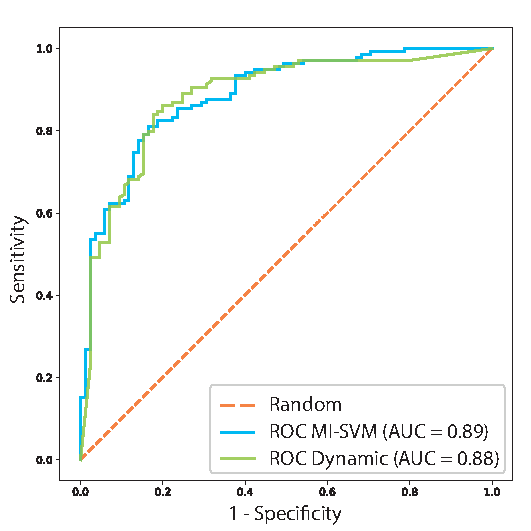
\includegraphics[width=\linewidth]{Figures/Result_Malignancy.pdf}
    \end{subfigure} 
    \begin{subfigure}{.45\linewidth}
        \centering
        \textbf{\ac{lm} \ac{roc} curves}\par
        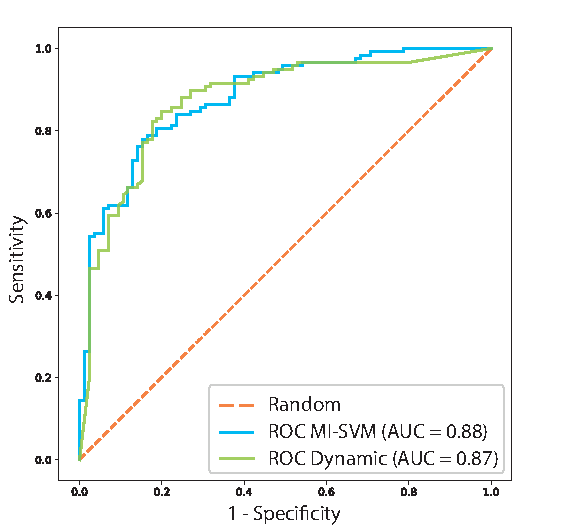
\includegraphics[width=\linewidth]{Figures/Result_LMM.pdf}
    \end{subfigure} 
    
    \caption{\ac{roc} curves from supervised methods based on Dynamic threshold method (as Dynamic) and multi-instance learning based on MI-SVM method (as MI-SVM). From left to right, the \ac{roc} curves for Malignancy and the \ac{roc} curves for \ac{lm}.}
    \label{fig:roc_results}
\end{figure}

%=====================================
% DISCUSSION
%=====================================
\section{Conclusions}
\label{sec:conclusions}
This research investigates the classification of malignant tumors and particularly \ac{lm} pathologies at image-level and at patient-level by use of \ac{rcm} images. First at the image-level, an analysis is performed over previous researches and proposed methods based on Transfer Learning are evaluated. Results show that “Inception-ResNet” architecture trained on the ImageNet database is quite relevant to classify the \ac{rcm} images with a weighted F1-Score of 0.83 between Benign and Malignant. Secondly at patient-level, proposed supervised decision methods are compared to \ac{mil} methods based on features extraction achieved with “Inception-ResNet” architecture. On the first hand, the classification of malignancy over patients achieves a weighted F1-Score of 0.84 with an \ac{auc} score of 0.88 using the supervised method based on a dynamic threshold. It achieves a weighted F1-Score of 0.82 with an \ac{auc} score of 0.89 using the \ac{mil} method based on MI-SVM. On the other hand, the classification of \ac{lm} over patient achieves a weighted F1-Score of 0.83 (Sensitivity 0.88 / Specificity 0.75) with an \ac{auc} score of 0.87 using the supervised method based on a dynamic threshold. It achieves weighted F1-Score of 0.80 (Sensitivity 0.78 / Specificity 0.84) with an \ac{auc} score of 0.88 using the \ac{mil} method based on MI-SVM. Both techniques are relevant compared to the evaluation of dermatologists, reaching 0.80 of sensitivity and 0.81 of specificity with an \ac{auc} score of 0.89. Furthermore, the supervised method based on the dynamic threshold has more sensitivity that can be relevant in the medical context.\par
Further steps of this work should focus on the enhancement of the image classification through improvement of the feature extraction process, in particular by investigating over fine-tuning of \ac{cnn} architecture. In another step, the patient decision should need to be improved by research on the score meaning through score calibration methods and change our approach the way the decision is taken through these.\par

% %%%%%%%%%%%%%%%%%%%%%%%%%%%%%%%%%%%%%%%%%%
% \vspace{6pt} 
\newpage

%%%%%%%%%%%%%%%%%%%%%%%%%%%%%%%%%%%%%%%%%%
\funding{This research was funded by the Conseil Regional de Bourgogne Franche-Comte, France and the European Regional Development Fund (ERDF).}

%%%%%%%%%%%%%%%%%%%%%%%%%%%%%%%%%%%%%%%%%%
\conflictsofinterest{The authors declare no conflict of interest.} 

%%%%%%%%%%%%%%%%%%%%%%%%%%%%%%%%%%%%%%%%%%
\acknowledgments{We thank Dr. Perrot and Dr. Cinotti for their work on the data and the permission granted to exploit it.\par}

%%%%%%%%%%%%%%%%%%%%%%%%%%%%%%%%%%%%%%%%%%
%% optional
\abbreviations{The following abbreviations are used in this manuscript:\\

\noindent 
\begin{tabular}{@{}ll}
\acs{auc}   & \Acl{auc}\\
\acs{bcc}   & \Acl{bcc}\\
\acs{cart}  & \Acl{cart}\\
\acs{cnn}   & \Acl{cnn}\\
\acs{dej}   & \Acl{dej}\\
\acs{ert}   & \Acl{ert}\\
\acs{ggd}   & \Acl{ggd}\\
\acs{glh}   & \Acl{glh}\\
\acs{glcm}  & \Acl{glcm}\\
\acs{lm}    & \Acl{lm}\\
\acs{mil}   & \Acl{mil}\\
\acs{rcm}   & \Acl{rcm}\\
\acs{roc}   & \Acl{roc}\\
\acs{sil}   & \Acl{sil}\\
\acs{svm}   & \Acl{svm}\\
\end{tabular}}

%=====================================
% References
%=====================================
\reftitle{References}
\externalbibliography{yes}
\bibliography{bibliography}

\end{document}

%%%%%%%%%%%%%%%%%%%%%%%%%%%%%%%%%%%%%%%%%%
%% optional
% \sampleavailability{Samples of the compounds ...... are available from the authors.}

%% for journal Sci
%\reviewreports{\\
%Reviewer 1 comments and authors’ response\\
%Reviewer 2 comments and authors’ response\\
%Reviewer 3 comments and authors’ response
%}

%%%%%%%%%%%%%%%%%%%%%%%%%%%%%%%%%%%%%%%%%%

% \begin{table}[h]
%     \centering
%     \begin{tabular}{lllll|lll}
%                                 &                   & \multicolumn{3}{c}{\textbf{Malignancy - F1-Score}}                    & \multicolumn{3}{c}{\textbf{\ac{lm} - F1-Score}}                       \\ \hline
%     \textbf{Category}           & \textbf{Name}     & \textbf{Weighted}     & \textbf{Benign}       & \textbf{Malignant}    & \textbf{Weighted}     & \textbf{Benign}       & \textbf{Malignant}    \\ \hline
%     \multirow{2}{*}{Decision}   & At Least One      & 0.61$\pm$0.06         & 0.32$\pm$0.07         & 0.79$\pm$0.05         & 0.58$\pm$0.07         & 0.32$\pm$0.07         & 0.76$\pm$0.06         \\ \cline{2-8} 
%                                 & \textbf{Dynamic}  & \textbf{0.84$\pm$0.03}& \textbf{0.78$\pm$0.07}& \textbf{0.87$\pm$0.02}& \textbf{0.83$\pm$0.03}& \textbf{0.79$\pm$0.06}& \textbf{0.86$\pm$0.03}\\ \hline 
%     \multirow{2}{*}{Score}      & Mean              & 0.83$\pm$0.03         & 0.78$\pm$0.08         & 0.87$\pm$0.02         & 0.82$\pm$0.03         & 0.79$\pm$0.07         & 0.85$\pm$0.01         \\ \cline{2-8}
%                                 & Maximum           & 0.76$\pm$0.04         & 0.68$\pm$0.03         & 0.80$\pm$0.05         & 0.74$\pm$0.04         & 0.69$\pm$0.03         & 0.78$\pm$0.06         \\ \hline  
%     \multirow{2}{*}{\ac{mil}}   & \ac{sil}          & 0.70$\pm$0.04         & 0.50$\pm$0.10         & 0.83$\pm$0.03         & 0.68$\pm$0.04         & 0.50$\pm$0.10         & 0.80$\pm$0.04         \\ \cline{2-8} 
%                                 & \textbf{MI-SVM}   & \textbf{0.82$\pm$0.02}& \textbf{0.78$\pm$0.05}& \textbf{0.84$\pm$0.02}& \textbf{0.80$\pm$0.03}& \textbf{0.78$\pm$0.05}& \textbf{0.82$\pm$0.03}\\ \hline 
%     \end{tabular}    
%     \caption{Results from patient-level classification for Malignancy(\ac{lm} and \ac{bcc}) and for \ac{lm} along the different proposed methods from \Cref{sec:patient_decision}. For Malignancy and \ac{lm}, the table provide a weighted average of F1-Score, and individual F1-Score for Benign and Malignant classes.}
%     \label{tab:patient_results}
% \end{table}\par